%\begin{figure}
%	\begin{tikzpicture}
%	\sbEntree{E}
%	\sbComp{a}{E}
%	\sbBloc{b}{P}{a}
%	\sbRelier[$x_{d}$]{E}{a}
%	\sbComp{c}{b}	
%	\sbRelier[$\epsilon_x$]{a}{b}
%	\sbRelier[$\dot{x}_{d}$]{b}{c}
%	
%	\sbBloc{d}{PI}{c}	
%	\sbRelier[$\epsilon_{\dot{x}}$]{c}{d}
%	
%	\sbComp{e}{d}	
%	\sbRelier[$I_d$]{d}{e}
%	
%	\sbBloc{f}{PI}{e}	
%	\sbRelier[$\epsilon_{I}$]{e}{f}
%	
%	
%	\sbBloc{g}{Process}{f}	
%	\sbRelier{f}{g}
%	
%	
%	\sbSortie{h}{g}
%	\sbRelier{g}{h}
%	
%	\sbRenvoi{g}{a}{$x_a$}
%	\sbRenvoi{g}{c}{$\dot{x}_a$}
%	\sbRenvoi{g}{e}{$I_a$}
%	
%	\draw [color=gray,thick](0,-2) rectangle (4.4,1.5);
%	\node at (0.5,1) [below=10mm, right=0mm] {sbRIO FPGA};
%	
%		\draw [color=gray,thick](4.4,-2) rectangle (10.75,1.5);
%		\node at (6.5,1) [below=10mm, right=0mm] {ESCON controller};
%	
%	\end{tikzpicture}
%	\caption{Embedded cascade control. x is position, $\dot{x}$ is speed, I is current. d index means demand, a index means actual value.}
%\end{figure}



\begin{figure}	 	
\resizebox{\textwidth}{!}{
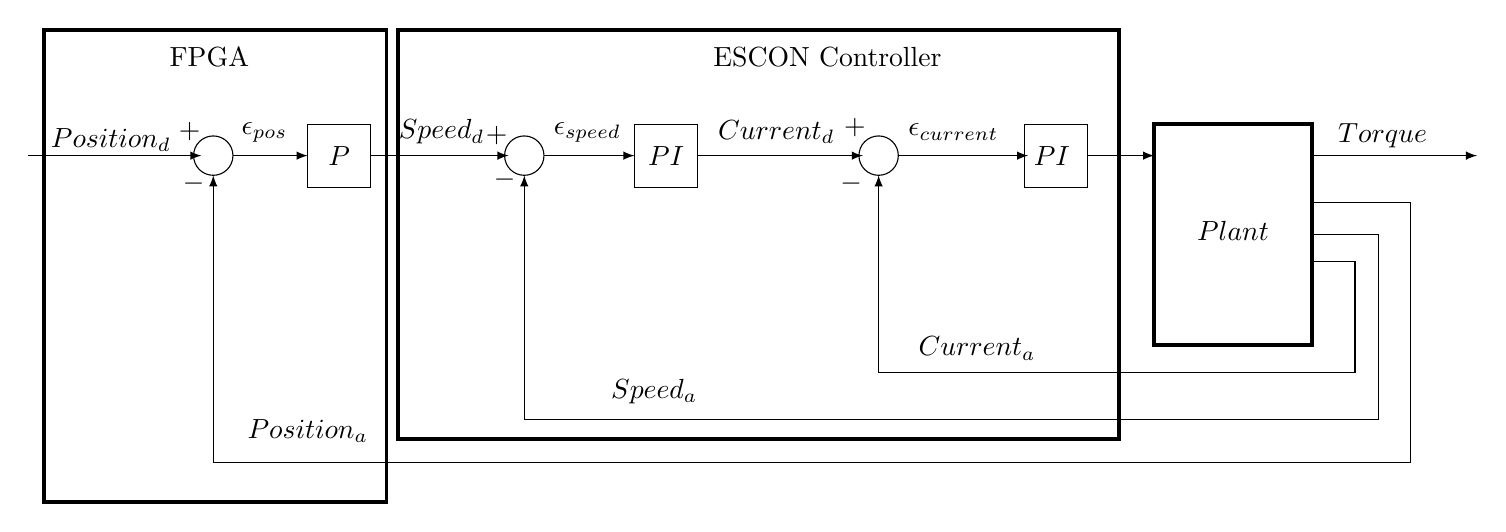
\begin{tikzpicture}%[transform canvas={scale=0.5}]

\draw [-latex] (10.6,3.4) ellipse (0.25 and 0.25);
\node at (7.9,3.4) {\normalsize{$PI$}};
\node at (12.8,3.4) {\normalsize{$PI$}};
\node at (17,3.65) {\normalsize{$Torque$}};
\node at (15.1,2.45) {\normalsize{$Plant$}};
\draw [-latex] (7.5,3.8) rectangle (8.3,3);
\draw [-latex] (12.45,3.8) rectangle (13.25,3);
\draw [-latex](8.3,3.4) -- (10.4,3.4);
\draw [-latex] (6.1,3.4) ellipse (0.25 and 0.25);
\draw [-latex](6.35,3.4) -- (7.5,3.4);
\node at (6.9,3.7) {$\epsilon_{speed}$};
\node at (11.55,3.7) {$\epsilon_{current}$};
\node at (3.75,3.4) {\normalsize{$P$}};
\draw [-latex] (3.35,3.8) rectangle (4.15,3);
\draw [-latex](4.15,3.4) -- (5.9,3.4);

\draw [-latex](10.85,3.4) -- (12.5,3.4);
\draw [-latex](13.25,3.4) -- (14.1,3.4);
\draw [-latex](16.1,3.4) -- (18.2,3.4);

\draw [-latex](16.1,2.05) -- (16.65,2.05) -- (16.65,0.65)-- (10.6,0.65)-- (10.6,3.15);
\draw [-latex](16.1,2.4) -- (16.95,2.4) -- (16.95,0.05)-- (6.1,0.05)-- (6.1,3.15);
\draw [-latex](16.1,2.8) -- (17.35,2.8) -- (17.35,-0.5)-- (2.15,-0.5)-- (2.15,3.15);

\node at (10.3,3.75) {$+$};
\node at (10.25,3.05) {$-$};

\draw [-latex] (2.15,3.4) ellipse (0.25 and 0.25);
\draw [-latex](2.4,3.4) -- (3.35,3.4);
\node at (5.85,3.1) {$-$};

\draw [-latex](-0.2,3.4) -- (2,3.4);
\node at (0.85,3.6) {$Position_d$};
\node at (2.1,4.65) {FPGA};
\node at (9.95,4.65) {ESCON Controller};
\node at (1.9,3.05) {$-$};
\node at (2.8,3.7) {$\epsilon_{pos}$};
\node at (5.05,3.7) {$Speed_d$};
\node at (9.3,3.7) {$Current_d$};
\node at (11.85,0.95) {$Current_a$};
\node at (7.75,0.4) {$Speed_a$};
\node at (3.35,-0.1) {$Position_a$};


\node (v2) at (1.85,3.7) {$+$};
\node (v2) at (5.75,3.65) {$+$};
\draw  [line width=0.5mm](14.1,3.8) rectangle (16.1,1);
\draw  [line width=0.5mm](0,5) rectangle (4.35,-1);
\draw [line width=0.5mm] (4.5,5) rectangle (13.65,-0.2);
\end{tikzpicture}
}
\caption{Embedded cascade control structure. d index means the desired control value, a index means actual value, $\epsilon$ is the error}
\label{cascade_fig}
\end{figure}
